\documentclass[../main-report.tex]{subfiles}
\begin{document}

\section{Hiện thực}
\subsection{Môi trường hiện thực}
Để thuận tiện trong việc đóng gói và triển khai ứng dụng, nhóm tác giả sử dụng công nghệ Container để hỗ trợ, đại diện tiêu biểu cho công nghệ Container mà nhóm tác giả chọn để sử dụng là Docker\footnote{https://www.docker.com}.

Công nghệ Docker container giúp người phát triển có thể triển khai ứng ở bất kì đâu miễn là có thể chạy được docker. Các ứng dụng được đóng gói trong container, có thể kiểm tra, xóa bất kì container. Các ứng dụng được triển khai dễ dàng và đồng nhất giữa các môi trường khác nhau.

Phiên bản docker và ứng dụng kèm theo mà nhóm tác giả triển khai bao gồm:

\begin{itemize}
\item \textbf{Docker Engine:} 19.03.3
\item \textbf{Docker Compose}: 1.21.0
\end{itemize}

\subsection{Các công nghệ được sử dụng}
Dựa vào kiến trúc hệ thống ở hình \ref{fig:system-architecture}, nhóm tác giả tiến hành chọn các công nghệ để hiện thực. Sơ đồ tổng quan về các công nghệ mà nhóm tác giả hiện thực được thể hiện ở hình \ref{fig:architecture-implementation}.

\begin{figure}[ht!]
\begin{center}
\label{fig:architecture-implementation}
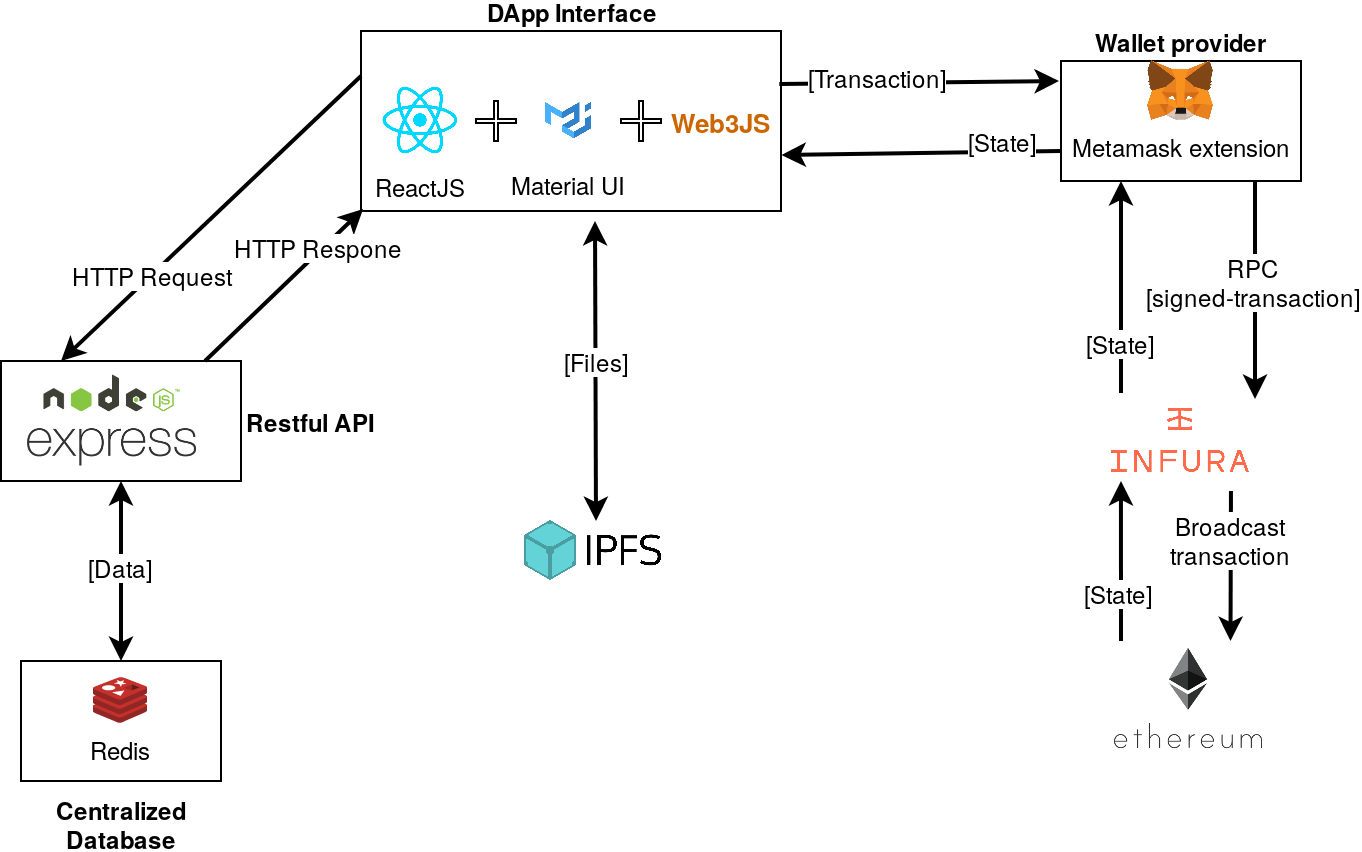
\includegraphics[scale=0.3]{architecture-implementation}
\caption{Sơ đồ hiện thực hệ thống}
\end{center}
\end{figure}

Các công nghệ được sử dụng bao gồm:
\begin{itemize}
\item Phần giao diện người dùng (\gls{frontend}): nhóm tác giả sử dụng \textbf{ReactJS/NodeJS} kết hợp \textbf{Material UI} để tạo giao diện ứng dụng web cho người dùng. Để tương tác với các hợp đồng thông minh, nhóm tác giả sử dụng thư viện Web3js và trình mở rộng Ví Metamask.
\item Phần \gls{backend} được chia làm hai thành phần như sau:
\begin{itemize}
 \item Kiến trúc phi tập trung (decentralized): nhóm sử dụng ngôn ngữ solidity để xây dựng các \gls{smartcontract} kết hợp \acrshort{ipfs} để thực hiện lưu trữ các dữ liệu phi tập trung.
 \item Kiến trúc tập trung (centralized): công nghệ NodeJS kết hợp với Redis để tổ chức và tương tác với dữ liệu tập trung.
 \end{itemize} 
\end{itemize}

Với hợp đồng thông minh và ngôn ngữ Solidity, nhóm tác giả sử dụng bộ công cụ Truffle framework để xây dựng và triển khai các mã hợp đồng thông minh.

\subsubsection{Công nghệ ReactJS/NodeJS}
\textbf{ReactJS} là một thư viện để hỗ trợ cho việc phát triển giao diện của người dùng. Đây là một trong những thư viện \gls{frontend} nổi tiếng với hơn $141.000$ sao đánh giá với hơn 2.8 triệu người dùng trên dịch vụ lưu trữ mã nguồn Github\footnote{https://github.com} (số liệu cập nhật tháng 12 năm 2019). Thư viện này được hỗ trợ và phát triển bởi Facebook\footnote{https://www.facebook.com} và Instagram\footnote{https://www.instagram.com} cùng với cộng đồng các nhà phát triển trên toàn thế giới và đang được phát triển từng ngày. ReactJS cung cấp tốt hơn về trải nghiệm người dùng và đồng thời có nhiều thư viện bên thứ ba hữu ích khác được phát triển kèm theo.

ReactJS được thiết kế và phát triển theo kiến trúc các component\footnote{là một kiểu kiến trúc trong phát triển phần mềm, chia ứng dụng ra thành các thành phần, bộ phận không phụ thuộc lẫn nhau và có thể tải sử dụng các thành phần này khi cần thiết}. Theo như tài liệu từ Facebook, định nghĩa React là một thư viện dành cho phát triển các mô đun cho giao diện người dùng. Về cơ bản, React cho phép các nhà lập trình phát triển các ứng dụng web lớn, phức tạp và đổng thời có thể thay đổi dữ liệu mà không cần tải lại trang. React sử dụng DOM ảo, điều này có tác dụng tăng hiệu suất kết xuất trang web, đồng thời nâng cao trải nghiệm của người dùng, cũng như rất dễ dàng lập trình phát triển sản phẩm.

\textbf{Node.js} hay còn được gọi là \textbf{Node} – là một nền tảng chạy trên môi trường Javascript hay còn được gọi là một nền tảng chạy trên môi trường V8 JavaScript runtime. Công nghệ V8 đã được triển khai hầu hết ở C và C++, công nghệ này tập trung chủ yếu vào hiệu suất và ít tiêu tốn bộ nhớ. Hầu hết V8 hỗ trợ chủ yếu Javascript trên trình duyệt (chú ý nhất là Google Chrome), mục đích hỗ trợ của Node đó chính là hỗ trợ các tiến trình có thời gian chạy dài. Không giống như những ngôn ngữ khác, Node không hỗ trợ đa luồng, nhưng hỗ trợ xử lý bất đồng bộ \cite{nodejs-performance}. Nhờ vào tính năng xử lý bất đồng bộ này, Node còn được biết đến là một nền tảng xử lý nhanh chóng hàng ngàn yêu cầu đồng thời, chịu tải cao, tốc độ thực thi và khả năng mở rộng tốt.

Đánh giá về hiệu suất của các ứng dụng chạy Node.js, nhóm tác giả có tham khảo nghiên cứu của tác giả Robert Ryan McCune về đo lường hiệu suất của ứng dụng Node.js \cite{mccune2011node}. Trong bài nghiên cứu, tác giả Robert Ryan McCune đã thực hiện phần đánh giá trên một máy ảo \textbf{Ubuntu 11.10} được tạo bởi VMWare Fusion 4.0.2 trên iMac \textit{OS X 10.6.8} với 8GB RAM và \textit{3.06Ghz Intel Core 2 Duo}, máy ảo này được được cấu hình với bộ nhớ là \textbf{2GB RAM}, và một bộ vi xử lý lõi kép. Tác giả đã thực hiện đồng thời 100 và 1000 yêu cầu đến máy chủ chạy bằng Node và thu được kết quả là thời gian trả lời từ máy chủ chưa tới 70ms. Tương tự thực hiện 500 yêu cầu đồng thời và thực hiện tổng cộng 10.000 yêu cầu thì thời gian phản hồi là dưới 140ms.

\subsubsection{Material UI framework}
\textbf{Material UI} là một thư viện được \textit{Google}\footnote{https://www.google.com} viết dành riêng cho ReactJS, bao gồm tập hợp nhiều các thành phần được xây dựng và thiết kế theo phong cách Material. Với hơn 52.8 nghìn sao đánh giá trên cộng đồng Github, và được sử dụng bởi hơn 139.000 dự án khác nhau, Material là một trong những thư viện UI được nhiều người sử dụng nhất trên thế giới. Giao diện của Material cũng tương đồng với các sản phẩm của Google như: \textit{Gmail, Google tìm kiếm, Google Form},\ldots

Material UI hiện tại cũng đang được sử dụng bởi \textit{NASA, UNIQLO, shutterstock},\ldots

Trong cuộc khảo sát vào năm 2019 của Oliver được đăng trên trang Medium\footnote{Nguồn: https://medium.com/material-ui/2019-material-ui-developer-survey-results-c9589434bbcf} đã chỉ ra rằng, có đến 74.4\% của 734 người khảo sát cho rằng sẽ thất vọng khi không còn sử dụng thư viện này. Biểu đồ thể hiện thái độ người khảo sát khi không còn được sử dụng thư viện Material ở hình \ref{fig:material-chart-survey}.

\begin{figure}[ht!]
\begin{center}
\label{fig:material-chart-survey}
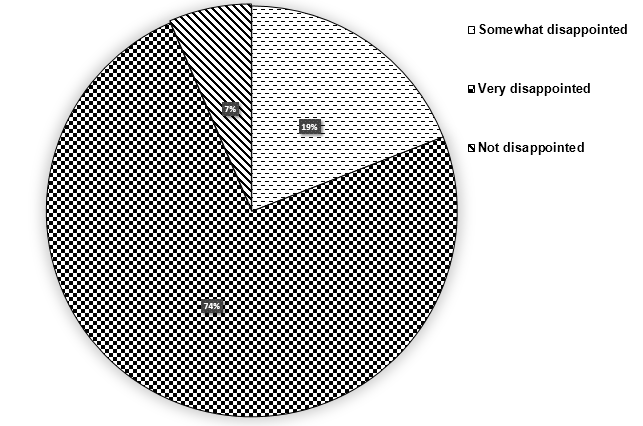
\includegraphics[scale=0.8]{material-chart-survey}
\caption{Biểu đồ thể hiện thái độ người dùng khi không còn được sử dụng thư viện Material}
\end{center}
\end{figure}

Cũng tại bài viết, tác giả đã ghi nhận nhận những lợi ích từ người khảo sát cho rằng yếu tố tập trung vào luồng xử lý, tiết kiệm thời gian, dễ dùng, \ldots và có đến 70\% dùng thư viện này để xây dựng dashboard, 40\% để thiết kế hệ thống, 35\% dùng để thiết kế các trang doanh nghiệp.

\subsubsection{Cơ sở dữ liệu Redis}
\textbf{Redis} là một cơ sở dữ liệu thường được xếp vào nhóm cơ sở dữ liệu NoSQL, được phát triển vào năm 2009. Khác với những cơ sở dữ liệu khác, Redis lưu dữ liệu trên RAM của máy chủ, điều này làm cho việc truy xuất giá trị nhanh hơn so với cách lưu trữ truyền thống – lưu trữ trên ổ cứng. Sau một thời gian, các bản ghi được lưu trên RAM này sẽ được lưu xuống ổ cứng nhằm tiết kiệm tài nguyên bộ nhớ RAM.

Các đặc điểm của Redis \cite{6106531}:

\begin{enumerate}[label=(\roman*)]
\item Redis là một dạng lưu trữ dữ liệu \textit{key-value}, như được nói ở trên khi Redis chạy, dữ liệu sẽ được lưu trữ trong bộ nhớ, do đó nó có thể xử lý hơn 100.000 thao tác đọc và ghi mỗi giây.
\item Redis hỗ trợ nhiều dạng lưu trữ như \textit{List} và \textit{Set},\ldots
\item Giá trị lớn nhất lưu trên Redis là 1GB.
\item Nhược điểm yếu nhất của Redis đó chính là dung lương của cơ sở dữ liệu bị giới hạn bởi bộ nhớ vật lý, do đó Redis không nên dùng làm cơ sở dữ liệu cho các dự án lớn và khả năng mở rộng kém.
\end{enumerate}

Với các đặc điểm trên, Redis phù hợp cho việc cung cấp hiệu suất cao cho lượng dữ liệu nhỏ.

\subsubsection{IPFS}
\textbf{\acrfull{ipfs}} là một giao thức chia sẻ tệp tin được phân tán ngang hàng \acrfull{p2p}. Giao thức này cho phép người dùng chia sẻ các tệp tin ngang hàng với nhau mà không cần có sự xuất hiện của máy chủ. Các dữ liệu khi người dùng tải lên sẽ được băm ra và đồng thời sinh ra mã băm của dữ liệu ấy. Với các dữ liệu giống nhau thì sẽ tạo ra những hàm băm giống nhau, do đó IPFS sẽ hạn chế được sự trùng lặp.
 
\acrshort{ipfs} có thể giải quyết vấn đề về lưu trữ dữ liệu lớn cho các ứng dụng \gls{blockchain} bằng cách sử dụng blockchain để lưu trữ địa chỉ của dữ liệu được ra bằng IPFS (chính là mã băm nhận diện cho tập tin) và đặt địa chỉ bất biến này cho một giao dịch trong blockchain. Không những giải quyết vấn đề lưu trữ, \acrshort{ipfs} còn giải quyết vấn đề về bằng thông bằng cách phân tán nội dung đến hệ thống \acrshort{p2p}. Do đó, khi truy cập tập tin nào đó bằng các dùng hàm băm, nút gần nhất với tệp sẽ phản hồi và gửi tệp cho người yêu cầu. Như đã được chứng minh từ trước \cite{5235364}, một hệ thống phân phát \acrshort{p2p} có thể tiết kiệm lên đến 60\% so với hệ thống truyền thống. Đồng thời, IPFS còn tăng tính bảo mật và chống lại các cuộc tấn công từ chối dịch vụ và giới hạn lại kiểm duyệt vì không có địa chỉ IP cụ thể của máy chủ bị chặn \cite{8441990}.

\subsubsection{Bộ công cụ Truffle framework}


\subsubsection{Thư viện web3js}


\subsubsection{Ví Metamask}


\subsection{Các bước hiện thực}
\begin{itemize}
\item Bước 1
\item Bước 2
\item Bước 3
\end{itemize}

\section{Đánh giá hệ thống đã hiện thực}
\subsection{Kiểm tra các quy trình trong hệ thống}


\subsection{Đo lường tốc độ thực hiện giao dịch}
Để tăng tính tin cậy cho phần đánh giá dưới đây của khóa luận, nhóm tác giả đã tham khảo mô hình đánh giá và kết quả đánh giá về hiệu suất của ethereum ở các công trình khác để làm thước đo và thực hiện tương tự với mô hình đánh giá đó.

Cụ thể, công trình của tác giả Sara Rouhani và Ralph Deters \cite{rouhani2017performance} đã đo được thời gian trung bình cho mỗi \gls{transaction} là 104.609ms với Parity client và 198.9125ms với Geth. Tổng số \gls{transaction} được gửi là 2000. Hai Ethereum private \gls{blockchain} khác nhau với cùng cấu hình được thực thi bởi Parity client và Geth client được sử dụng để đo lường. Cấu hình hệ thống bao gồm 24GiB RAM và Core i7-6700 CPU. Việc gửi các \gls{transaction} được thực hiện bằng ngôn ngữ NodeJS và sau đó thu thập thời gian xử lí cho việc xác nhận các \gls{transaction}.

\subsubsection{Môi trường thực hiện đánh giá}
Nhóm tác giả thực hiện việc đánh giá này trên cấu hình máy như sau:

\begin{itemize}
\item \textbf{CPU}: 4 x Intel(E) Pentium(R) CPU N3540 @ 2.16GHz
\item \textbf{RAM}: 8GB
\item \textbf{OS}: Alpine Linux 3.9 running in Docker container
\end{itemize}

Công cụ mà nhóm tác giả sử dụng trong phần đánh giá này là \textbf{Truffle framework}\footnote{https://www.trufflesuite.com}, đây là một bộ công cụ được sử dụng để triển khai các hợp đồng thông minh hỗ trợ ngôn ngữ Solidity.

Trong phần đánh giá thời gian này, nhóm tác giả sử dụng một mạng ethereum riêng được chạy trên mạng cục bộ nhằm loại bỏ đi thời gian chờ xác nhận giao dịch thông thường trên các mạng công khai hiện tại.

\subsubsection{Phương pháp thực hiện đánh giá}
Đầu tiên nhóm tác giả thực hiện lựa chọn các hàm trong hợp đồng thông minh thường xuyên được sử dụng trong hệ thống, sau đó các hàm được chọn sẽ được hiện thực thông qua các \gls{transaction}. Các \gls{transaction} sẽ được xử lí và gửi đi bằng NodeJS, thời gian đo được tính từ lúc \gls{transaction} được tạo ra đến lúc hoàn tất \gls{transaction} đó. Với mỗi \gls{transaction}, thực hiện gửi đi tuần tự 100, 200, 400, 600, 900 lần với cùng một bộ tham số cho trước. Sau đó lấy kết quả là thời gian trung bình thực hiện cho mỗi \gls{transaction}.

Các hàm được chọn và tham số đầu vào cho mỗi hàm để đo thời gian được thể hiện ở bảng \ref{tab:listfunction-timeperform}.

\begin{table}[!ht]
\centering
\resizebox{\textwidth}{!}{%
\begin{tabular}{|l|l|l|l|}
\hline
\multicolumn{1}{|c|}{\textbf{Contract}} & \multicolumn{1}{c|}{\textbf{Hàm được chọn}} & \multicolumn{1}{c|}{\textbf{Tham số đầu vào}}                                                                                                                                                                                                                           & \multicolumn{1}{c|}{\textbf{Ghi chú}}                    \\ \hline
Wallet                                  & deposit()                                   &                                                                                                                                                                                                                                                                         & value  = $10^{15}$ gas                      \\ \hline
\multirow{3}{*}{Campaigns}              & createCampaign()                            & \begin{tabular}[c]{@{}l@{}}77760000,\\ 1000000,\\ 1,\\ {[}{]},\\ 0,\\ {[}{]},\\ '8f1ef45972ebd8ef45b2410e8a0b399181fed3d929738d2eb96baf470758a97d',\\ 'c2337a3217ffcf3b01398d83577a1c32235ceb4f481b8c7be00a055798e95d36'\end{tabular}                                   & \begin{tabular}[c]{@{}l@{}}tạo chiến dịch\\với số giai đoạn\\giải ngân $= 1$\end{tabular}            \\ \cline{2-4} 
                                        & createCampaign()                            & \begin{tabular}[c]{@{}l@{}}77760000,\\ 1000000,\\ 3,\\ {[}300000, 300000, 400000{]}\\ 2,\\ {[}0, 7200, 7200{]},\\'8f1ef45972ebd8ef45b2410e8a0b399181fed3d929738d2eb96baf470758a97d',\\ 'c2337a3217ffcf3b01398d83577a1c32235ceb4f481b8c7be00a055798e95d36'\end{tabular} & \begin{tabular}[c]{@{}l@{}}tạo chiến dịch\\với số giai đoạn\\giải ngân $> 1$\end{tabular} \\ \cline{2-4} 
                                        & donate()                                    & \begin{tabular}[c]{@{}l@{}}0,\\ 1\end{tabular}                                                                                                                                                                                                                          &                                                          \\ \hline
\end{tabular}%
}
\caption{Các hàm và tham số đầu vào được dùng để đo thời gian thực hiện giao dịch}
\label{tab:listfunction-timeperform}
\end{table}

\subsubsection{Kết quả đánh giá}
Sau khi thực hiện đánh giá thời gian, nhóm tác giả đã tổng hợp kết quả như ở bảng \ref{tab:result-timeperform}. Theo như kết quả tổng hợp được, nhóm tác giả nhận xét rằng với dữ liệu đầu vào càng nhiều (kích thước lớn) thì thời gian xử lí càng lâu.

% Please add the following required packages to your document preamble:
% \usepackage{multirow}
% \usepackage{graphicx}
\begin{table}[!ht]
\centering
\resizebox{\textwidth}{!}{%
\begin{tabular}{|l|l|l|l|l|l|l|l|l|}
\hline
\multicolumn{1}{|c|}{\textbf{Contract}} & \multicolumn{1}{c|}{\textbf{Hàm}} & \multicolumn{1}{c|}{\textbf{\begin{tabular}[c]{@{}c@{}}Thời gian\\ thực hiện\\ 100 lần\\ (giây)\end{tabular}}} & \multicolumn{1}{c|}{\textbf{\begin{tabular}[c]{@{}c@{}}Thời gian\\ thực hiện\\ 200 lần\\ (giây)\end{tabular}}} & \multicolumn{1}{c|}{\textbf{\begin{tabular}[c]{@{}c@{}}Thời gian\\ thực hiện\\ 400 lần\\ (giây)\end{tabular}}} & \multicolumn{1}{c|}{\textbf{\begin{tabular}[c]{@{}c@{}}Thời gian\\ thực hiện\\ 600 lần\\ (giây)\end{tabular}}} & \multicolumn{1}{c|}{\textbf{\begin{tabular}[c]{@{}c@{}}Thời gian\\ thực hiện\\ 900 lần\\ (giây\end{tabular}}} & \multicolumn{1}{c|}{\textbf{\begin{tabular}[c]{@{}c@{}}Thời gian\\ trung bình\\ (giây)\end{tabular}}} & \multicolumn{1}{c|}{\textbf{Ghi chú}}                            \\ \hline
Wallet                                  & deposit                           & 11.099                                                                                                         & 18.035                                                                                                         & 36.484                                                                                                         & 54.166                                                                                                         & 86.968                                                                                                        & 0.095856                                                                                              &                                                                  \\ \hline
\multirow{3}{*}{Campaigns}              & createCampaign                    & 19.613                                                                                                         & 37.839                                                                                                         & 76.577                                                                                                         & 115.433                                                                                                        & 172.447                                                                                                       & 0.1921527                                                                                             & \begin{tabular}[c]{@{}l@{}}một g.đoạn\\ giải ngân\end{tabular}   \\ \cline{2-9} 
                                        & createCampaign                    & 31.986                                                                                                         & 63.561                                                                                                         & 127.236                                                                                                        & 191.94                                                                                                         & 287.694                                                                                                       & 0.319063                                                                                              & \begin{tabular}[c]{@{}l@{}}nhiều g.đoạn\\ giải ngân\end{tabular} \\ \cline{2-9} 
                                        & donate                            & 16.529                                                                                                         & 32.083                                                                                                         & 63.9                                                                                                           & 94.204                                                                                                         & 142.934                                                                                                       & 0.160255                                                                                              &                                                                  \\ \hline
\end{tabular}%
}
\caption{Bảng kết quả đánh giá thời gian hiện thực một số hàm trong hệ thống.}
\label{tab:result-timeperform}
\end{table}

Từ kết quả thu được, ta có biểu đồ tổng quan về tốc độ thực hiện của các hàm như ở hình \ref{fig:result-time-perform-chart}.

\begin{figure}[ht!]
\begin{center}
\label{fig:result-time-perform-chart}
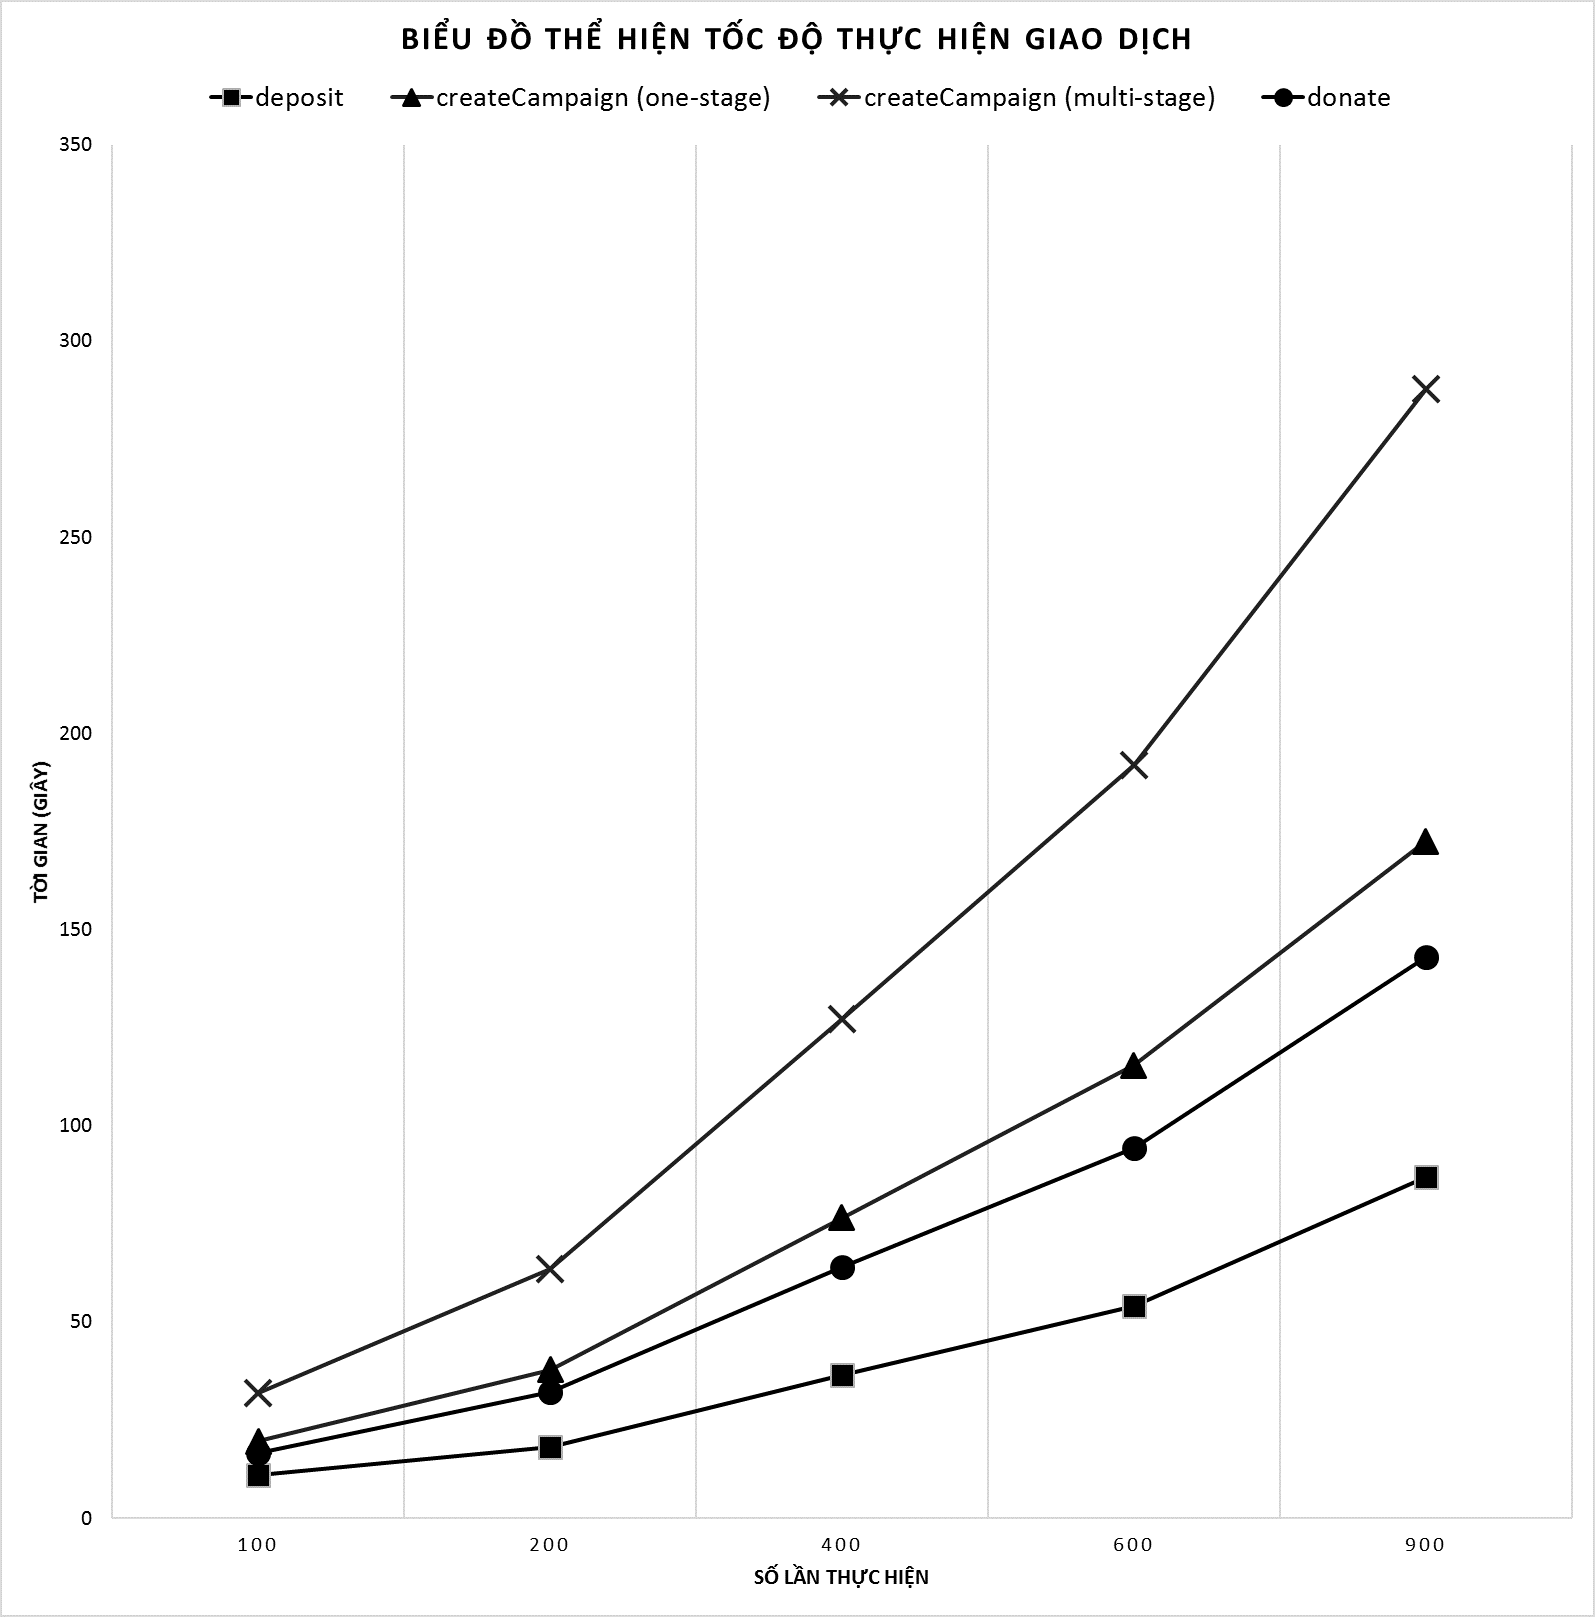
\includegraphics[scale=0.5]{result-time-perform-chart}
\caption{Biểu đồ thể hiện tốc độ thực hiện giao dịch giữa các hàm}
\end{center}
\end{figure}

Nhìn vào kết quả, ta thấy được:

\begin{itemize}
\item Hàm \textit{deposit} là hàm có tốc độ thực hiện nhanh nhất với thời gian trung bình là 0.095856 giây. Phần mã xử lí của hàm deposit tương đối ngắn nên thời gian xử lí nhanh hơn.
\item Hàm có tốc độ xử lí chậm nhất là hàm \textit{createCampaign} (với chiến dịch gây quỹ có nhiều giai đoạn giải ngân). Do hàm này có tham số đầu vào tương đối nhiều và phần mã lí phức tạp hơn nên thời gian hoàn tất lâu hơn những hàm khác.
\end{itemize}
\subsection{Chi phí thực hiện các giao dịch trong hệ thống}
\subsubsection{Môi trường thực hiện đánh giá}
Nhóm tác giả thực hiện việc đo lường chi phí giao dịch trên cấu hình máy như sau:

\begin{itemize}
\item \textbf{CPU}: 4 x Intel(E) Pentium(R) CPU N3540 @ 2.16GHz
\item \textbf{RAM}: 8GB
\item \textbf{OS}: Alpine Linux 3.9 running in Docker container
\end{itemize}

Bộ công cụ \textbf{Truffle framework} kết hợp plug-in có tên là \textbf{eth-gas-reporter}\footnote{https://www.npmjs.com/package/eth-gas-reporter} được sử dụng để triển khai các hợp đồng thông minh và đo lường chi phí thực hiện. Mạng ethereum riêng chạy trên máy cục bộ được sử dụng nhằm loại bỏ đi thời gian chờ xác nhận giao dịch thông thường trên các mạng công khai hiện tại.
\subsubsection{Phương pháp thực hiện đánh giá}
Do chỉ có các hàm thực hiện ghi dữ liệu mới tốn chi phí thực hiện nên nhóm tác giả chọn ra các hàm có thao tác ghi dữ liệu, sau đó các hàm được chọn sẽ được hiện thực thông qua các \gls{transaction}. Các \gls{transaction} sẽ được xử lí và gửi đi bằng NodeJS. Sau đó thực hiện ghi lại kết quả chi phí.

Các hàm được chọn và tham số đầu vào cho mỗi hàm để đo lường chi phí được thể hiện ở bảng \ref{tab:input-cost-perform}. Các tham số đầu vào mẫu được cho là sát với thực tế khi triển khai hệ thống (độ dài từng tham số mẫu là sát với thực tế).

\begin{table}[!ht]
\centering
\resizebox{\textwidth}{!}{%
\begin{tabular}{|l|l|l|l|}
\hline
\multicolumn{1}{|c|}{\textbf{Contract}} & \multicolumn{1}{c|}{\textbf{Hàm}} & \multicolumn{1}{c|}{\textbf{Dữ liệu đầu vào}}                                                                                                                                                                                                                                                                                                                                                  & \multicolumn{1}{c|}{\textbf{Ghi chú}}                                                                \\ \hline
\multirow{2}{*}{Wallet}                 & deposit                           &                                                                                                                                                                                                                                                                                                                                                                                                & \begin{tabular}[c]{@{}l@{}}Thực hiện gửi\\ vào 2000 tokens\end{tabular}                              \\ \cline{2-4} 
                                        & withdraw                          & 1000                                                                                                                                                                                                                                                                                                                                                                                           &                                                                                                      \\ \hline
\multirow{4}{*}{Identity}               & addVerify                         & \begin{tabular}[c]{@{}l@{}}'0x93598a39777ED4B4Af3Ac7429d123Ca3bE9658C5',\\ 'AAAAB3NzaC1yc2EAAAADAQABAAAAgQCDxbho2O3XWhktz4Hwi6/61ltfk/l\\ SCqeXLufvjr6O3wh1++MmTZT+KzcO0azsKsiFJTXL7ynC06Vp1Hp9o0BK3Q/Q\\ ZTo8jRoP3XX1LBu1CLe7OeOA5P2TO/nz2mWtuxz0b11GmRrjO8YoznizlPiolL\\ kv9hoDBvwTy0JonyJ6+w=='\end{tabular}                                                                                &                                                                                                      \\ \cline{2-4} 
                                        & changePubKey                      & \begin{tabular}[c]{@{}l@{}}'0x93598a39777ED4B4Af3Ac7429d123Ca3bE9658C5',\\ 'MIGfMA0GCSqGSIb3DQEBAQUAA4GNADCBiQKBgQCMjs5j52lzXN6XX+nZ1js\\ yaBgzVBsA/JlWVux1zL0pw4GocvqPsZrIKwKsTeQycGdf3azjKRKwMga6g8fPF\\ HO+Ayh+6v33B1h+3ckWu81alwsM+Y9ADpcMret5qH2Mv9rDyWi+lmAYeUA\\ OOosAWfmgc6QJz+psSMtuGKOr08q+1wIDAQAB'\end{tabular}                                                                    &                                                                                                      \\ \cline{2-4} 
                                        & registerIdentity                  & \begin{tabular}[c]{@{}l@{}}'KLTN',\\ 'UIT-HCM, Linh Trung, Thu Duc, HCM',\\ 830550240,\\ 'QmarHSr9aSNaPSR6G9KFPbuLV9aEqJfTk1y9B8pdwqK4Rq',\\ 'frPULs0boASMCqSq1guu+jX636wkY+fzhFSRnFQi9dQuK50yzCobUIGm5b/f7\\ oGDea/NrieB5c883EpWiQdgJlO+0B43jJLAtfSfJ/mlbGX3FUPc6LAQzxlCb5FSh\\ 7+Q1E4WIUyFwLwoNdipDYFcpuXxtCsKeepjFHwGFhfupxM=',\\ '0x93598a39777ED4B4Af3Ac7429d123Ca3bE9658C5'\end{tabular} &                                                                                                      \\ \cline{2-4} 
                                        & verify                            & \begin{tabular}[c]{@{}l@{}}'0x41A418C946Fd3201b7b2b30B367De35b0c54A6ce',\\ true\end{tabular}                                                                                                                                                                                                                                                                                                   &                                                                                                      \\ \hline
\multirow{7}{*}{Campaigns}              & createCampaign                    & \begin{tabular}[c]{@{}l@{}}77760000,\\ 1000000,\\ 1,\\ {[}{]},\\ 0,\\ {[}{]},\\ '8f1ef45972ebd8ef45b2410e8a0b399181fed3d929738d2eb96baf470758a97d',\\ 'c2337a3217ffcf3b01398d83577a1c32235ceb4f481b8c7be00a055798e95d36'\end{tabular}                                                                                                                                                          & \begin{tabular}[c]{@{}l@{}}tạo chiến dịch\\ với số giai đoạn\\ giải ngân = 1\end{tabular}            \\ \cline{2-4} 
                                        & createCampaign                    & \begin{tabular}[c]{@{}l@{}}10,\\ 1000,\\ 3,\\ {[}300, 300, 400{]},\\ 0,\\ {[}{]},\\ '8f1ef45972ebd8ef45b2410e8a0b399181fed3d929738d2eb96baf470758a97d',\\ 'c2337a3217ffcf3b01398d83577a1c32235ceb4f481b8c7be00a055798e95d36'\end{tabular}                                                                                                                                                      & \begin{tabular}[c]{@{}l@{}}tạo chiến dịch\\ với số giai đoạn\\ giải ngân \textgreater 1\end{tabular} \\ \cline{2-4} 
                                        & verifyCampaign                    & \begin{tabular}[c]{@{}l@{}}1,\\ true\end{tabular}                                                                                                                                                                                                                                                                                                                                              &                                                                                                      \\ \cline{2-4} 
                                        & donate                            & \begin{tabular}[c]{@{}l@{}}1,\\ 1000\end{tabular}                                                                                                                                                                                                                                                                                                                                              &                                                                                                      \\ \cline{2-4} 
                                        & claimRefund                       & \begin{tabular}[c]{@{}l@{}}1,\\ 200\end{tabular}                                                                                                                                                                                                                                                                                                                                               &                                                                                                      \\ \cline{2-4} 
                                        & donate                            & \begin{tabular}[c]{@{}l@{}}1,\\ 200\end{tabular}                                                                                                                                                                                                                                                                                                                                               & \begin{tabular}[c]{@{}l@{}}thực hiện donate\\ lại cho đủ mục\\ tiêu chiến dịch\end{tabular}          \\ \cline{2-4} 
                                        & endCampaign                       & 1                                                                                                                                                                                                                                                                                                                                                                                              &                                                                                                      \\ \hline
Disbursement                            & vote                              & \begin{tabular}[c]{@{}l@{}}1,\\ 1,\\ true\end{tabular}                                                                                                                                                                                                                                                                                                                                         &                                                                                                      \\ \hline
\end{tabular}%
}
\caption{Các hàm và dữ liệu đầu vào được dùng để đo lường chi phí giao dịch}
\label{tab:input-cost-perform}
\end{table}

\subsubsection{Kết quả chi phí cho các giao dịch trong hệ thống}
Bảng tổng hợp chi phí cho các giao dịch được liệt kê ở bảng \ref{tab:result-cost-perform}. Kết quả màn hình khi chạy chạy công cụ đo lường chi phí được thể hiện ở hình \ref{fig:result-perform-cost-1}.

\begin{figure}[ht!]
\begin{center}
\label{fig:result-perform-cost-1}
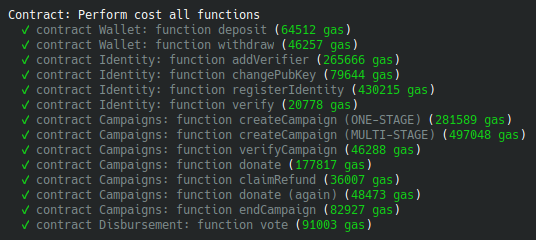
\includegraphics[scale=0.8]{result-perform-cost-1}
\caption{Ảnh chụp màn hình kết quả đo lường chi phí giao dịch}
\end{center}
\end{figure}

Công cụ đo lường còn cung cấp cho chúng ta chi phí triển khai các hợp đồng thông minh, kết quả được thể hiện ở bảng \ref{tab:result-cost-deployment}.

Một số đại lượng trong bảng kết quả:

\begin{itemize}
\item \textbf{Gas} - là một đơn vị đo lường công việc tính toán của các giao dịch hoặc hợp đồng thông minh trong mạng Ethereum.
\item \textbf{ETH} - là một đơn vị tiền tệ được sử dụng nội bộ trong mạng Ethereum. Tỉ lệ trao đổi giữa các đại lượng như sau: giá gas là 2 GWei/gas, và 1 ETH = $10^9$ GWei. Giá trị chuyển đổi giữa ETH và USD hiện tại được tham khảo trên \textbf{CoinMarketcap}\footnote{https://coinmarketcap.com} là 150.08 USD/ETH (cập nhật ngày 27/11/2019)
\end{itemize}

% Please add the following required packages to your document preamble:
% \usepackage{multirow}
\begin{table}[!ht]
\centering
\begin{tabular}{|l|l|l|l|l|}
\hline
\multicolumn{1}{|c|}{\textbf{Contract}} & \multicolumn{1}{c|}{\textbf{Hàm}} & \multicolumn{1}{c|}{\textbf{\begin{tabular}[c]{@{}c@{}}Chi phí\\ tính toán\\ (gas)\end{tabular}}} & \multicolumn{1}{c|}{\textbf{\begin{tabular}[c]{@{}c@{}}Chi phí\\ giao dịch\\ (ETH)\end{tabular}}} & \multicolumn{1}{c|}{\textbf{\begin{tabular}[c]{@{}c@{}}Chi phí\\ giao dịch\\ (USD)\end{tabular}}} \\ \hline
\multirow{2}{*}{Wallet}                 & deposit                           & 64512                                                                                             & 0.000129024                                                                                       & 0.02                                                                                              \\ \cline{2-5} 
                                        & withdraw                          & 46257                                                                                             & 0.000092514                                                                                       & 0.01                                                                                              \\ \hline
\multirow{4}{*}{Identity}               & addVerify                         & 265666                                                                                            & 0.000531332                                                                                       & 0.08                                                                                              \\ \cline{2-5} 
                                        & changePubKey                      & 79644                                                                                             & 0.000159288                                                                                       & 0.02                                                                                              \\ \cline{2-5} 
                                        & registerIdentity                  & 430215                                                                                            & 0.000860430                                                                                       & 0.13                                                                                              \\ \cline{2-5} 
                                        & verify                            & 20778                                                                                             & 0.000041556                                                                                       & 0.01                                                                                              \\ \hline
\multirow{7}{*}{Campaigns}              & createCampaign                    & 281589                                                                                            & 0.000563178                                                                                       & 0.08                                                                                              \\ \cline{2-5} 
                                        & createCampaign                    & 497048                                                                                            & 0.000994096                                                                                       & 0.15                                                                                              \\ \cline{2-5} 
                                        & verifyCampaign                    & 46288                                                                                             & 0.000092576                                                                                       & 0.01                                                                                              \\ \cline{2-5} 
                                        & donate                            & 177817                                                                                            & 0.000355634                                                                                       & 0.05                                                                                              \\ \cline{2-5} 
                                        & claimRefund                       & 36007                                                                                             & 0.000072014                                                                                       & 0.01                                                                                              \\ \cline{2-5} 
                                        & donate                            & 48473                                                                                             & 0.000096946                                                                                       & 0.01                                                                                              \\ \cline{2-5} 
                                        & endCampaign                       & 82927                                                                                             & 0.000165854                                                                                       & 0.02                                                                                              \\ \hline
Disbursement                            & vote                              & 91003                                                                                             & 0.000182006                                                                                       & 0.03                                                                                              \\ \hline
\end{tabular}
\caption{Kết quả đo lường chi phí giao dịch}
\label{tab:result-cost-perform}
\end{table}


\begin{table}[!ht]
\centering
\begin{tabular}{|l|l|l|l|}
\hline
\multicolumn{1}{|c|}{\textbf{Contract}} & \multicolumn{1}{c|}{\textbf{\begin{tabular}[c]{@{}c@{}}Chi phí\\ (gas)\end{tabular}}} & \multicolumn{1}{c|}{\textbf{\begin{tabular}[c]{@{}c@{}}Chi phí\\ (ETH)\end{tabular}}} & \multicolumn{1}{c|}{\textbf{\begin{tabular}[c]{@{}c@{}}Chi phí\\ (USD)\end{tabular}}} \\ \hline
Campaigns                               & 3447461                                                                               & 0.006894922                                                                           & 1.03                                                                                  \\ \hline
Disbursement                            & 1331555                                                                               & 0.002663110                                                                           & 0.4                                                                                   \\ \hline
Identity                                & 2401480                                                                               & 0.004802960                                                                           & 0.72                                                                                  \\ \hline
Wallet                                  & 1163284                                                                               & 0.002326568                                                                           & 0.35                                                                                  \\ \hline
\end{tabular}
\caption{Kết quả đo lường chi phí triển khai các hợp đồng}
\label{tab:result-cost-deployment}
\end{table}

Đánh giá tổng quan về chi phí:

\begin{itemize}
\item Hàm \textit{verify} trong contract Identity có mức chi phí thực hiện thấp nhất với 20778 gas (tương đương 0.000041556 ETH). Phần mã xử lí của hàm này tương đối ngắn nên chi phí thấp hơn.
\item Hàm có chi phí cao nhất là hàm \textit{createCampaign} (tạo chiến dịch với nhiều giai đoạn) với chi phí 497048 gas (tương đương 0.000994096 ETH). Do hàm này có tham số đầu vào tương đối nhiều và phần mã lí phức tạp hơn nên chi phí cao hơn những hàm khác.
\item Contract \textit{Campaigns} có chi phí triển khai cao nhất (3447461 gas), contract có chi phí triển khai thấp nhất là \textit{Identity} với 1163284 gas.
\end{itemize}
\subsection{Phân tích bảo mật của hợp đồng thông minh trong hệ thống}

\subsection{Đánh giá tốc độ tải trang của giao diện người dùng}
\subsubsection{Môi trường thực hiện}
Thông tin cấu hình máy sử dụng để đo tốc độ truy xuất của ReactJS như sau:

\begin{itemize}
\item Trình duyệt Google Chrome version 78.0.3904 (được cài sẵn extension MetaMask đã cấp phép truy cập thông tin)
\item Chip xử lý: 2.7 Ghz Dual-Core intel Core i5
\item HĐH: macOS Catalina version 10.15.1
\item RAM: 8GB 1867Mhz DDR3
\item Graphics: Intel Iris Graphics 6100 1536 MB
\end{itemize}
\subsubsection{Kết quả đánh giá}
Kết quả được tổng hợp ở bảng \ref{tab:result-perform-ui}.

% Please add the following required packages to your document preamble:
% \usepackage{graphicx}
\begin{table}[!ht]
\centering
\resizebox{\textwidth}{!}{%
\begin{tabular}{|l|l|l|l|l|l|l|l|}
\hline
\multicolumn{1}{|c|}{\textbf{Page}} & \multicolumn{1}{c|}{\textbf{Loading}} & \multicolumn{1}{c|}{\textbf{Scripting}} & \multicolumn{1}{c|}{\textbf{Rendering}} & \multicolumn{1}{c|}{\textbf{Painting}} & \multicolumn{1}{c|}{\textbf{System}} & \multicolumn{1}{c|}{\textbf{Idle}} & \multicolumn{1}{c|}{\textbf{Total}} \\ \hline
Detail campaign                     & 28 ms                                 & 1320 ms                                 & 70 ms                                   & 65 ms                                  & 220 ms                               & 918 ms                             & 2621 ms                             \\ \hline
Home page                           & 6 ms                                  & 743 ms                                  & 3 ms                                    & 3 ms                                   & 41 ms                                & 102 ms                             & 898 ms                              \\ \hline
Create campaign                     & 24 ms                                 & 1181 ms                                 & 47 ms                                   & 36 ms                                  & 196 ms                               & 672 ms                             & 2156 ms                             \\ \hline
Explore campaigns                   & 14 ms                                 & 798 ms                                  & 98 ms                                   & 82 ms                                  & 237 ms                               & 1541 ms                            & 2770 ms                             \\ \hline
\end{tabular}%
}
\caption{Bảng kết quả đo tốc độ truy xuất front-end của hệ thống}
\label{tab:result-perform-ui}
\end{table}
\end{document}